\documentclass[12pt, letterpaper]{article}

% =====================
% Paquetes
% =====================
\usepackage[utf8]{inputenc}
\usepackage[T1]{fontenc}
\usepackage[spanish]{babel}
\usepackage{lmodern}
\usepackage{setspace}
\usepackage[hyphens]{url}
\usepackage{amsmath}
\usepackage{geometry}
\usepackage{longtable}
\usepackage{booktabs}
\usepackage{fancyhdr}
\usepackage{array}
\usepackage{multirow}
\usepackage[table]{xcolor}
\usepackage{titlesec}
\usepackage{float}
\usepackage{graphicx}
\usepackage{caption}
\usepackage{csquotes}
\usepackage[style=apa, backend=biber]{biblatex}
\addbibresource{referencias.bib} % Archivo de bibliografía
\usepackage{xcolor}
\usepackage{hyphenat}
\usepackage{ragged2e} 
\usepackage{placeins}
\geometry{margin=1in}
\setlength{\parindent}{1.27cm}
\setlength{\parskip}{1em}
\onehalfspacing

% Configuración títulos
\titleformat{\section}{\normalfont\bfseries\uppercase}{\thesection.}{1em}{}
\titleformat{\subsection}{\normalfont\bfseries}{\thesubsection.}{1em}{}
\renewcommand{\contentsname}{Índice}

% Encabezados y pies
\pagestyle{fancy}
\fancyhf{}
\fancyfoot[C]{\thepage}

\newfloat{cuadro}{htbp}{loc}
\floatname{cuadro}{Cuadro}
\makeatletter
\let\c@cuadro\c@table % hace que 'cuadro' use el mismo contador que 'table'
\makeatother

% =====================
% Documento
% =====================
\let\cleardoublepage\clearpage
\begin{document}

% Portada
\begin{titlepage}
    \centering
    \includegraphics[width=5cm]{../logo_universidad.png}\par
    \vspace{1cm}
    
    {\bfseries\LARGE Quinta entrega: Matriz de verificación, Matriz de supuestos y MML\par}
        \vspace{2cm}
    {\large Autores: Jorge Luis Araque, Juan Camilo Velasquez, Juan David Tabares, Jhoan Esteban Corrales, Juan Esteban Cardona, Maicol Stiven Ruiz y Santiago Marin\par}
    {\large Docente: Alexánder Quintero\par}
    \vfill
    {\Large Facultad de Ingenierías, Universidad Tecnológica de Pereira \par}
    {\large Curso: Gerencia de Proyectos\par}
    {\large Pereira, Colombia \\ \today \par}
\end{titlepage}

\renewcommand{\contentsname}{Tabla de contenido}
% Índice
\tableofcontents
\newpage

\section{Matriz de supuestos}

\begin{figure}[H]
    \centering
    \includegraphics[width=1\linewidth]{images/supuestos.png}
    \caption{Matriz de supuestos}
    \vspace{0.2cm}
    \small Fuente: Elaboración propia
    \label{fig:supuestos}
\end{figure}

\section{Matriz de medios de verificación}

\begin{figure}[H]
    \centering
    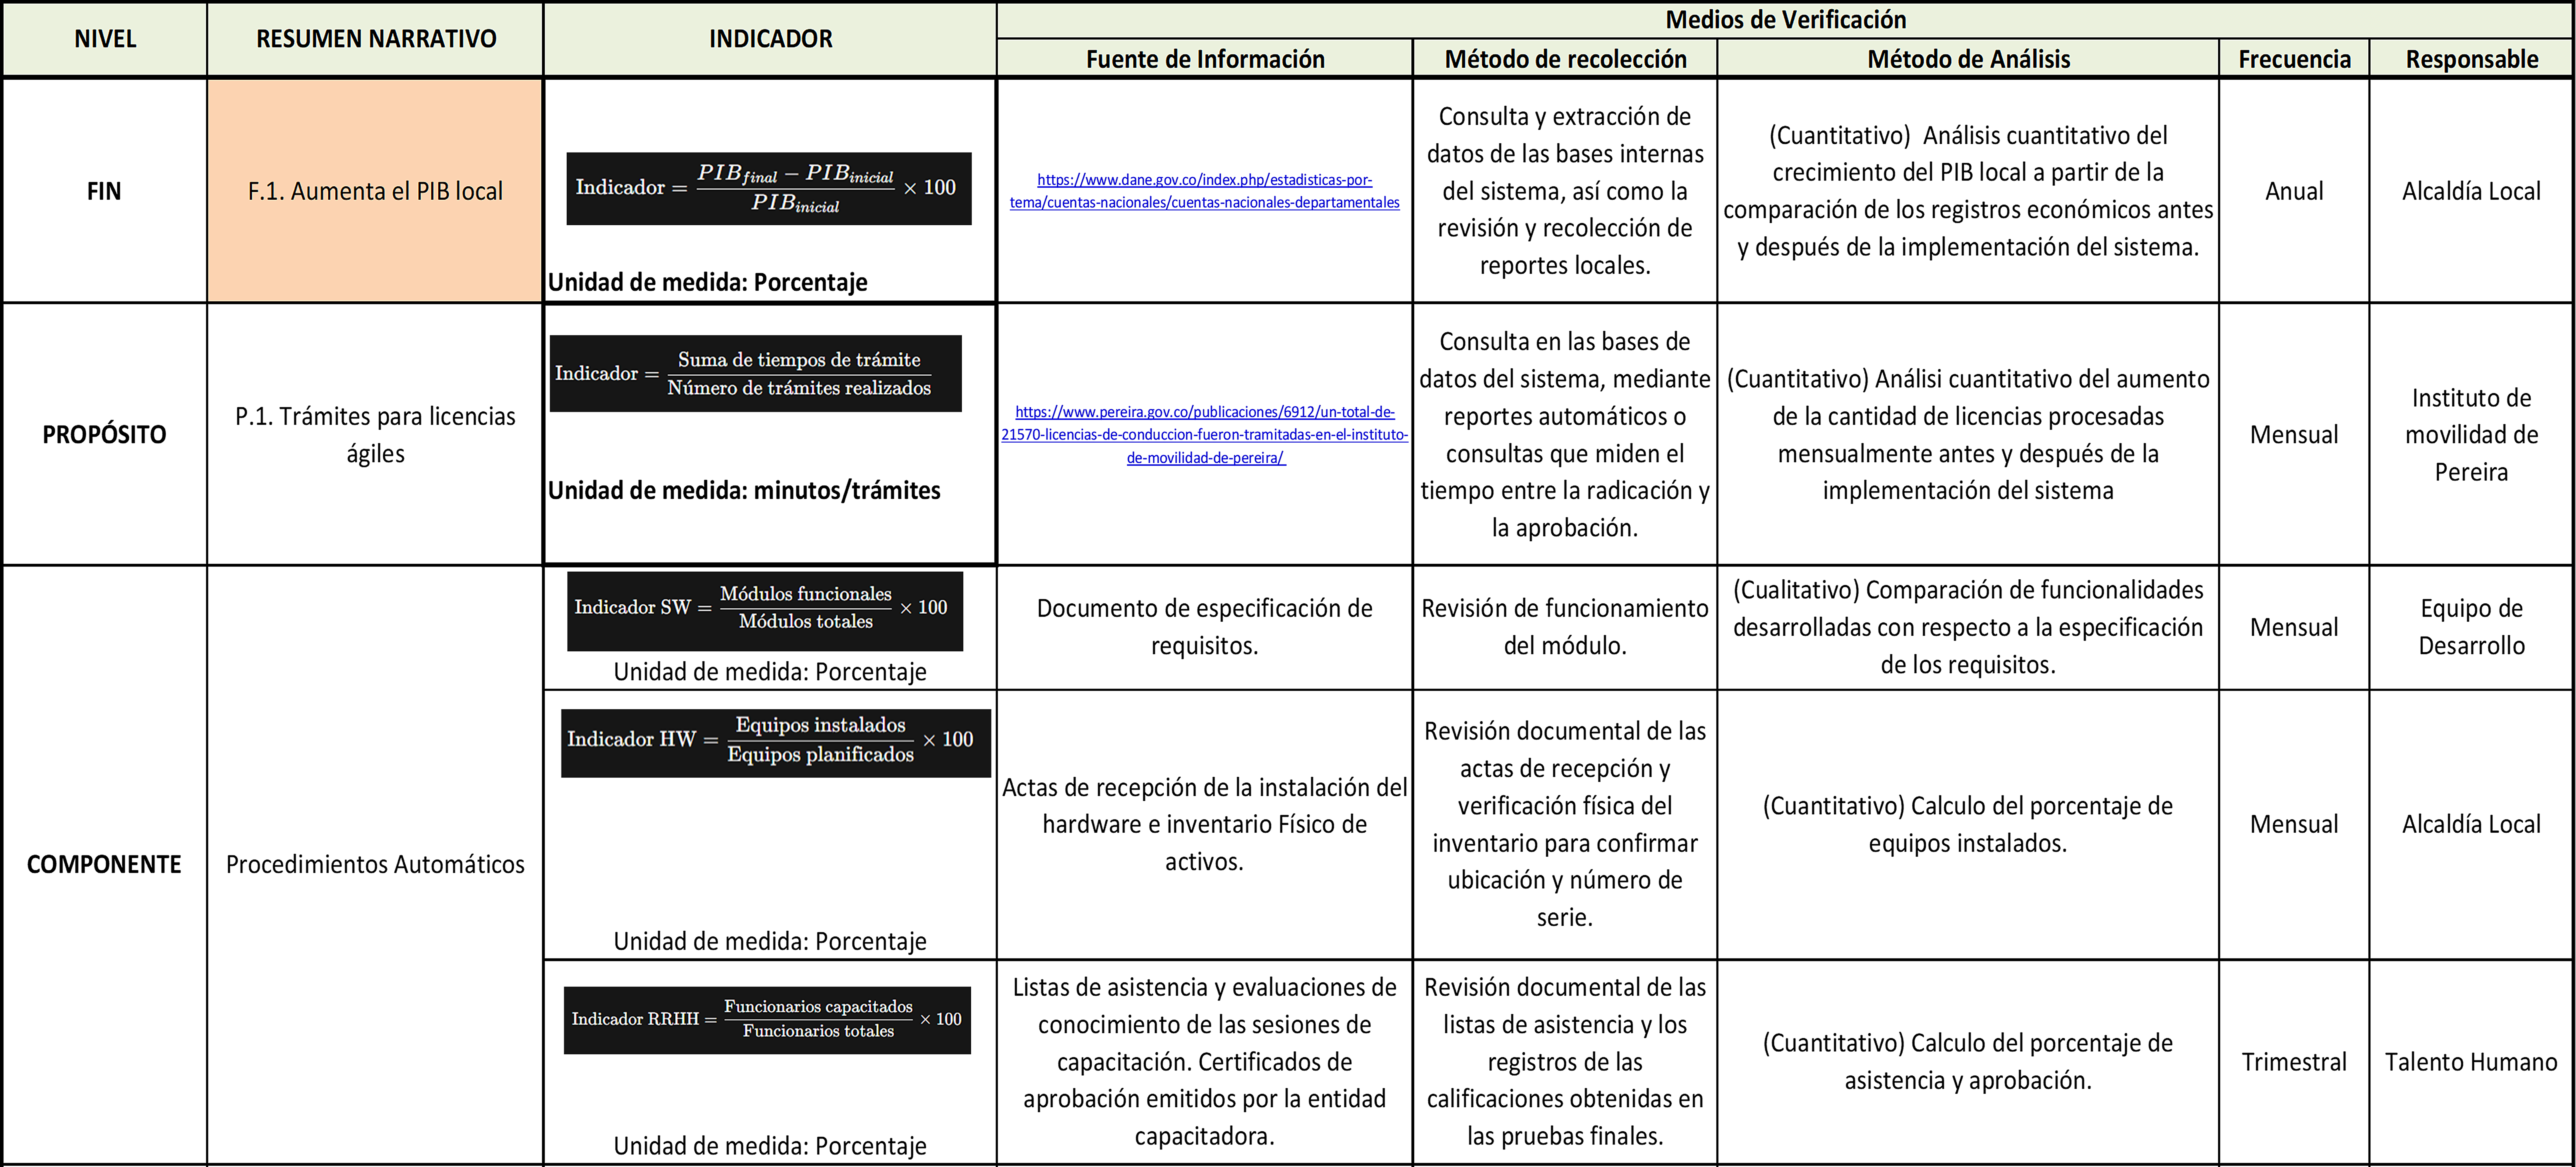
\includegraphics[width=1\linewidth]{images/verificacion1.png}
    \caption{Matriz de medios de verificación - parte 1}
    \vspace{0.2cm}
    \small Fuente: Elaboración propia
    \label{fig:medios de verificación1}
\end{figure}


\begin{figure}[H]
    \centering
    \includegraphics[width=1\linewidth]{images/verificacion2.png}
    \caption{Matriz de medios de verificación - parte 2}
    \vspace{0.2cm}
    \small Fuente: Elaboración propia
    \label{fig:medios de verificación2}
\end{figure}

\section{Matriz de Marco Lógico}

\begin{figure}[H]
    \centering
    \includegraphics[width=1\linewidth]{images/mml1.png}
    \caption{Matriz de Marco Lógico - parte 1}
    \vspace{0.2cm}
    \small Fuente: Elaboración propia
    \label{fig:mml1}
\end{figure}


\begin{figure}[H]
    \centering
    \includegraphics[width=1\linewidth]{images/mml2.png}
    \caption{Matriz de Marco Lógico - parte 2}
    \vspace{0.2cm}
    \small Fuente: Elaboración propia
    \label{fig:mml2}
\end{figure}

\end{document}